\documentclass[12pt]{report}
\usepackage[a4paper, width=150mm, top=25mm, bottom=25mm, headheight=20mm]{geometry}
\usepackage[backend=biber, style=numeric, sorting=none]{biblatex}
\usepackage{graphicx}
\usepackage{fancyhdr}
\usepackage{parskip}
\usepackage{xcolor}
\usepackage{soul}  % For highlighting text - remove when done
\usepackage{hyperref}
\usepackage[explicit,compact]{titlesec}
\usepackage{pdfpages}
\hypersetup{colorlinks=true, linkcolor=black, citecolor=black, urlcolor=blue}
\graphicspath{{./images/}}
\counterwithout{figure}{chapter}
\addbibresource{citations.bib}
\titleformat{\chapter}[block]{\bfseries\huge}{\filright\huge\thechapter.}{1ex}{\huge\filright #1}
\titlespacing*{\section}{0pt}{5.5ex plus 1ex minus .2ex}{3.3ex plus .2ex}

\renewcommand{\chaptermark}[1]{\markboth{#1}{}}

% For highlighting text - remove when done
\newcommand{\hlc}[2][yellow]{{%
    \colorlet{foo}{#1}%
    \sethlcolor{foo}\hl{#2}}%
}

\pagestyle{fancy}
\fancyhead[L]{From Scramble to Solution}
\fancyhead[R]{\leftmark}
\fancyfoot[C]{\thepage}

\title{From Scramble to Solution: Developing an Optimal Solver for the Kilominx, a Rubik's Cube Variant}
\author{Samuel Borg}
\date{\today}

\begin{document}

\begin{titlepage}
    \begin{center}
        \vspace*{1.5cm}
            
        \Huge
        \textbf{From Scramble to Solution}
            
        \vspace{0.5cm}
        \LARGE
        Developing an Optimal Solver for \\ the Kilominx, a Rubik's Cube Variant

        \vspace{2cm}
        \textbf{Samuel Borg}

        \Large
        \textit{Supervisor: Ian Gent}

        \vspace{0.5cm}

        \large
        \today

        \vspace{2.5cm}

        
\includegraphics[width=0.4\textwidth]{unilogo}

        \Large
        \vspace{0.5cm}
        School of Computer Science\\
        University of St Andrews
    \end{center}
\end{titlepage}

\chapter*{Abstract}
The Rubik's Cube is the most well-known combination puzzle of all time, and has inspired numerous variants of the puzzle. One such puzzle is the Kilominx, a 2x2 dodecahedron-shaped puzzle with 12 faces and 20 cubies (individual cube elements of the puzzle). While the Rubik's Cube has already been extensively researched, the Kilominx has not.

This report details my work in creating an optimal solver for the Kilominx, guaranteeing solutions in as few moves as possible. A separate program I wrote precomputes several pattern databases, each containing the number of moves required to solve different subsets of cubies in all possible states. The solver uses an iterative-deepening A* (IDA*) algorithm to find the optimal solution, using the pattern databases as a lower-bound heuristic. In order to efficiently index into the pattern databases, the solver computes a Lehmer code for the puzzle state, which is then used to calculate the state's sequential index.

In theory, the solver could optimally solve any state given enough time, but in practice it can only find solutions up to a depth of 14 within a reasonable timeframe. As solutions require longer sequences of moves to solve, the solver takes exponentially more time to find the optimal solution. Results from the solver demonstrate that it is unlikely an optimal solver could be used to help tighten the bounds on the Kilominx's God's Number - the maximum number of moves needed to solve the puzzle from any given state.

\chapter*{Declaration}
I declare that the material submitted for assessment is my own work except where credit is explicitly given to others by citation or acknowledgement. This work was performed during the current academic year except where otherwise stated.

The main text of this project report is \hlc[yellow]{[insert word count]} words long, including project specification and plan.

In submitting this project report to the University of St Andrews, I give permission for it to be made available for use in accordance with the regulations of the University Library. I also give permission for the title and abstract to be published and for copies of the report to be made and supplied at cost to any bona fide library or research worker, and to be made available on the World Wide Web. I retain the copyright in this work.

\chapter*{Acknowledgements}
I would like to thank my supervisor, Ian Gent, for his invaluable guidance, insight and support throughout this project. His expertise and enthusiasm have made this project an incredibly engaging and rewarding journey.

I would also like to thank my parents, Juliet and Peter, my brother, Tom, and my amazing friends Emil, Ben, Zoe, Josh, Maya, Jess and Alfie for their unwavering support and belief in me all the way through my studies.

\tableofcontents

\chapter{Introduction}
% Describe the problem you set out to solve and the extent of
% your success in solving it. You should include the aims and
% objectives of the project in order of importance and try to
% outline key aspects of your project for the reader to look for
% in the rest of your report.

When the Rubik's Cube was globally released in 1980, it became an instant success, selling around 200 million units by the end of 1983 \cite{unitssold}. The Rubik's Cube also quickly became a popular subject of research for computer scientists, in part due to the massive 43 quintillion possible states \cite{states} that the cube can be in. Many different algorithms were designed to try and solve the cube in as few a number of moves as possible, but it wasn't until 1997 that Richard E. Korf published a paper \cite{korf} describing a method to solve the Rubik's Cube optimally (the shortest possible number of moves to solve any given cube state) by using large lookup tables called pattern databases\cite{patterndatabases} as a heuristic function to guide an IDA* search algorithm. 

% god number stuff here

The widespread success of the Rubik's Cube also led to the creation of a number of different variants of the puzzle, each working similarly to the Rubik's Cube but of different shapes and sizes. The Kilominx is one of these variants, part of the larger "minx" family of dodecahedron-shaped puzzles. The Kilominx is a 2x2 dodecahedral puzzle with 12 faces and 20 cubies (the individual cube-shaped elements of the puzzle). Although some research has been done on tightening the bounds of its God's Number, no optimal solver has previously been created for the puzzle.

\begin{figure}[h]
    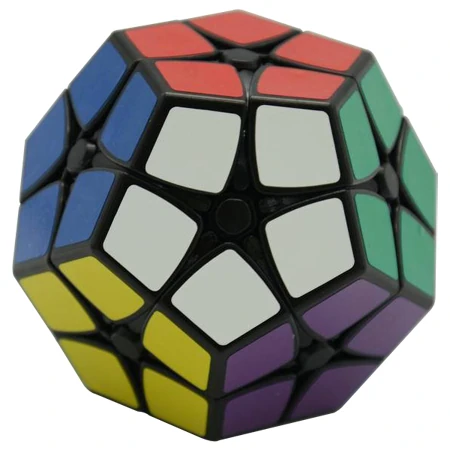
\includegraphics[width=0.4\textwidth]{kilominx}
    \centering
    \caption{An image of a Kilominx.}
    % Image URL: https://static.wikia.nocookie.net/speedcubesolving/images/8/88/4941_P_1467693201156-1-.jpg/revision/latest?cb=20180218173628
    % Website URL: https://speedcubesolving.fandom.com/wiki/Kilominx
\end{figure}

\section{Objectives}

\chapter{Context Survey}
% Surveying the context, the background literature and any
% recent work with similar aims. The context survey describes
% the work already done in this area, either as described in
% textbooks, research papers, or in publicly available software.
% You may also describe potentially useful tools and
% technologies here but do not go into project-specific
% decisions.

\section{Korf's Algorithm for the Rubik's Cube}
% Go into detail about Korf's paper for the rubik's cube. Mention any important design decisions he made. Relate it to what I am doing.
\subsection{Iterative-Deepening A*}
\subsection{Pattern Databases}
% Small section here about the other pattern databases paper. Why use pattern databases?

\subsection{Sequential Indexing with Lehmer Codes}
% Again, more here to do with sequential indexing and lehmer codes. Use Korf's other paper, and possibly the article that explains it.

\section{God's Number}
% What research has been done on God's Number for the cube and the kilominx? What methods were used? How does it relate to what I'm doing?

\section{The Kilominx}
% Any research on the Kilominx?

\chapter{Requirements Specification}
% Capturing the properties the software solution must have in
% the form of requirements specification. You may wish to
% specify different types of requirements and given them
% priorities if applicable.

\chapter{Software Engineering Process}
\section{Software Development Process}
An incremental development process was used for this project in order to ensure steady progress throughout both semesters. This approach allowed me to slowly build up the solver in small, functional increments, where each increment was thoroughly tested and documented before moving on to the next. This method helped ensure that the final solution was robust and well-documented.

At the start of the project, I began by creating a reference guide for creating an optimal solver for the Rubik's Cube. This guide detailed each of the steps required to model the Rubik's Cube and then create the optimal solver for it, highlighting any important design decisions that needed to be made along with concise justifications for the decisions. This guide was used as a roadmap for the development of the solver, ensuring that I stayed on track towards the final goal.

After creating the reference guide, I followed it to implement an optimal solver for the Rubik's Cube. While creating a solver for the Rubik's Cube was not part of the project objectives, it was a necessary step in order to gain a better understanding of the process required to create an optimal solver. I took care while implementing the classes and methods to ensure that they were modular and reusable - this allowed me to easily extend the both the solver and other classes to work with the Kilominx later on. The Rubik's Cube solver was thoroughly tested to ensure that it was working correctly before moving on to implementing the Kilominx solver.

Finally, I implemented the Kilominx solver following the same steps from the reference guide as I did for the Rubik's Cube solver. I reused many of the classes and methods from the Rubik's Cube solver, extending them where necessary to work with the Kilominx. The Kilominx solver was also thoroughly tested to ensure that it was working correctly.

\section{Choice of Language}
I decided to use Java as the primary programming language for the solver. This decision was made based on my familiarity with Java and its object-oriented principles, such as abstract classes and inheritance, which I believed would be helpful for allowing parts of the code to be reused and extended. Additionally, Java is a relatively fast language and is well-suited for the type of computation required for solving the Rubik's Cube and Kilominx. There was some consideration given to using C++ due to its speed and efficiency, but due to my lack of experience with the language, I ultimately decided that Java would be the best choice for this project.


\chapter{Ethics}
The original project objectives involved surveying users about their experience with the web application, so the Artefact Evaluation form was filled out and submitted. However, as this objective was moved down to a lower priority, the user survey was ultimately not conducted. The Artefact Evaluation form can be found in \textbf{\hyperref[appendix:artefact]{Appendix A}}.

\chapter{Design}
% Indicating the structure of the system, with particular focus
% on main ideas of the design, unusual design features, etc.

\section{Design Overview}
% Quick overview of layout of classes (inheritance, abstract classes, etc)

\section{Representing State}
% Talk about using an array of Cubies (index + orientation) to represent the state of the cube/kilominx
% Why do it this way?
% How does the order of the array matter?
% What does "orientation" mean? How do we use it to get the colours?

\section{Making Moves}
% Talk about making moves on the cube/kilominx, and briefly talk about the idea of skipping moves to reduce search
% For kilominx, talk about fixing a cubie in one position, and how this affects the moves

\section{Populating Pattern Databases}
% Talk about the design of the pattern databases themselves, and how they are populated via search
% How did I choose which cubies for the pattern databases?

\section{Lehmer Codes}
% Talk about using Lehmer codes to calculate database indices - full maths section here

\section{Searching for Solutions}
% Talk about IDA* search

\section{Interacting with the Puzzles}
% Quick talk about terminal/GUI classes
% Talk about editing the puzzles, and the checks to ensure input is valid

\chapter{Implementation}
% How the implementation was done and tested, with
% particular focus on important / novel algorithms and/or data
% structures, unusual implementation decisions, novel user
% interface features, etc.

% Use of Enums and Consts?

% Talk about things done for efficiency
% - Using bytes instead of ints
% - Direct array manipulation

% How did I implement the Lehemer code computation?
% How did I make it efficient?

% Pattern database classes - N and K? Size? Rank calculations?
% For kilominx, draw attention to how the fixed cubie is NOT counted

% PDB population - BFS vs IDDFS?

% Solver - IDA*? How to use the PDBs as a heuristic?

% UI - displaying puzzle state? editing?
% GUI?

% Testing?

\chapter{Evaluation}
% You should evaluate your own work with respect to your
% original objectives. You should also critically evaluate your
% work with respect to related work done by others. You
% should compare and contrast the project to similar work in
% the public domain, for example as written about in published
% papers, or as distributed in software available to you. 

\section{Experimental Results}

\section{Evaluation Against Objectives}

\section{Comparison to Existing Work}

\chapter{Conclusions}
% You should summarise your project, emphasising your key
% achievements and significant drawbacks to your work, and
% discuss future directions your work could be taken in.

\appendix
\chapter{Artefact Evaluation Form}
\label{appendix:artefact}
\includepdf[pages=1]{ethics.pdf}

\chapter{Testing Summary}
% This should describe the steps taken to debug, test, verify or
% otherwise confirm the correctness of the various modules
% and their combination.

\chapter{User Manual}
% Instructions on installing, executing and using the system
% where appropriate.

\printbibliography[heading=bibintoc, title={References}]

\end{document}
